
\chapter{Reconnaissance basée sur l'extraction de \nfw{features}}




Si l'utilisation des données brutes comme entrée des réseaux de neurones 
permet déjà d'obtenir des résultats encourageant, il est possible de faire 
mieux en effectuant un pré-traitement des données. 
Il s'agit d'extraire des données brutes (i.e.\/ les pixels de l'image) des 
caractéristiques (ou \nfw{features} en anglais) qui permettent de décrire 
l'image dans un format plus adapté pour une machine.

\newcommand{\features}{\nfw{features}}
Ces \features peuvent être regroupés en deux catégories : 
\begin{enumerate}
  \item les \features statistiques, qui vont s'intéresser à des densité de pixels, 
  des extremums et autres transformées mathématiques;
  \item les \features structurelles, qui s’intéressent aux traits (strokes), aux courbes,
  aux nombres de bifurcations, etc…, ces dernières sont plus intuitives pour l’humain.
\end{enumerate}

Nous allons dans ce chapitre présenter quelques \features qui peuvent être 
utilisées dans le cadre de la reconnaissance de caractères. Puis nous les utiliserons 
comme entrées de différents algorithmes de \nfw{machine learning}.



\section{Binarisation de l'image}



Les images du jeu de données sont en niveaux de gris. 
C'est à dire que chaque pixel est représenté par un entier entre 0 
et 255 (du blanc au noir). 
Certains algorithmes ne prennent pas en compte le niveau de coloration 
du pixel et s'intéresse juste au fait que le pixel soit noir ou blanc. 
Il est donc utile, dans ce cas de binariser l'image (i.e.\/ de passer 
à la convention 0 pour un pixel ne contenant pas d'encre et 1 pour 
un pixel en contenant). 
On choisit donc arbitrairement un seuil à partir duquel on considère que 
le pixel est colorié.

\begin{codeblock}
def binarize(img, treshold = 200):
    w = len(img)
    h = len(img[0])
    ret = img.copy()
    for x in range(w):
        for y in range(h):
            ret[y][x] = 1 if img[y][x] >= treshold else 0
    return ret
\end{codeblock}

Bien évidemment, le choix du seuil peut avoir un impact sur le calcul des 
\features si l'on choisit un seuil très élevé, beaucoup de pixels seront 
considérés comme vide. A contrario, si le seuil est très faible, on considéra 
qu'un pixel est colorié dès qu'il y aura un peu d'encre dessus, ce qui peut 
également poser des problèmes.



\section{Densités de pixels coloriés}



\section{Nombre de croissements (\nfw{crossings})}



On prend deux points à l’extrémité de l’image et on compte le nombre d’alternance 
entre les groupes de pixels vides et les groupes de pixels contenant de l’encre. 
Cette méthode n’est à priori pas sensible à l’épaisseur du trait.



\section{Histogramme des projections}



On compte pour chaque ligne (resp. chaque colonne) le nombre de pixels allumés sur 
la ligne (resp. colonne). 
En faisant ça sur l’ensemble de l’image, on obtient deux histogrammes. 
Cette technique peut aussi être utilisé pour segmenter des lignes et caractères isolés. 
Cette technique peut être sensible à l’épaisseur du trait. 
Pour palier ce problème, on peut renormaliser chaque histogramme en divisant 
chaque valeur par le total.

\begin{figure}[h]
  \centering
  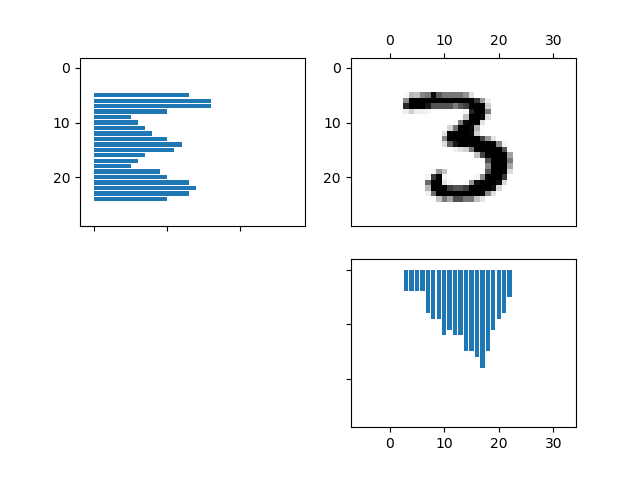
\includegraphics[scale=0.5]{assets/features-hvhisto-ex1}
  \caption{Histogramme des projections du chiffre 3.}
  \label{fig:features-hvhisto-ex1}
\end{figure}



\section{Moments}



Dans tout ce qui suit, on note $p_{xy}$ la valeur du pixel $(x,y)$.

On définit le moment d'ordre $(p+q)$ par:
\[
m_{pq} = \sum_x \sum_y x^p y^q p_{xy}
\]

En pratique, on préférera utiliser des moments centrés (car invariant 
par translation de l'image).
\[
\mu_{pq} = \sum_x \sum_y (x - \overline{x})^p (y - \overline{y})^q p_{xy}
\]
avec 
\[
\overline{x} = \frac{m_{10}}{m_{00}} \qquad \qquad \overline{y} = \frac{m_{01}}{m_{00}}
\]



\section{Transformée de Fourier du contour}



\section{Transformée de Fourier de l'image}